\documentclass[a4paper, 12pt]{article}
%\documentclass{book}

% Important Packages:
 \usepackage{amsmath}    % need for subequations
 \usepackage{amsfonts}
 \usepackage{amsthm}
 \usepackage{graphicx}   % need for figures
 \usepackage{verbatim}   % useful for program listings
 %\usepackage{subfig}  % use for side-by-side figures
 %\usepackage{wrapfig}
 %\usepackage{listings}	 % creates code blocks
 %\usepackage[colorlinks=true]{hyperref}   % use for hypertext links, including
                     % those to external documents and URLs
 %\usepackage{multirow}
 %\usepackage{tikz}
 %\usepackage{enumerate}
 %\usetikzlibrary{decorations.pathreplacing,decorations.pathmorphing}
 %\usetikzlibrary{calc}
 %\usepackage[colorinlistoftodos]{todonotes}
 \usepackage{tikz,tkz-euclide}
 \usepackage{float}
 
 \usetikzlibrary{calc,patterns,angles,quotes}
\usetkzobj{all}

\def\deg{^{\circ}}
\newcommand\heading[1]{\ \\\large{\textbf{#1}}}
\newcommand\ora[1]{\overrightarrow{#1}}

\def\thm{Th\textsuperscript{\underline{m}}}

%------------------end---preamble--------------------
 
 % Useful macros 
 \def\tcb#1{\color{blue}{#1}}
 \def\tcr#1{\color{red}{#1}}	
 \def\tcg#1{\color{green}{#1}}
 \def\be{\begin{eqnarray}}	 	\def\ee{\end{eqnarray}}
 \def\bea{\begin{eqnarray}}	 	\def\eea{\end{eqnarray}}
 \def\bean{\begin{eqnarray*}}	\def\eean{\end{eqnarray*}}
 
 \def\D{\displaystyle}
 \def\T{\textstyle}
 \def\l{\left}
 \def\r{\right}
 \def\nf{n_{\!f}} % quark flavours
 \def\pa{\partial}
 \def\eg{e.\,g.}
 \def\ie{i.\,e.}

 \def\be{\begin{equation}}
 \def\ee{\end{equation}}
 \def\bea{\begin{eqnarray}}
 \def\eea{\end{eqnarray}}
 \def\bean{\begin{eqnarray*}}
 \def\eean{\end{eqnarray*}}
 \def\gsim{\mathrel{\rlap{\lower0.2em\hbox{$\sim$}}\raise0.2em\hbox{$>$}}}
 \def\ksim{\mathrel{\rlap{\lower0.2em\hbox{$\sim$}}\raise0.2em\hbox{$<$}}}
 \def\kg{\mathrel{\rlap{\lower0.25em\hbox{$>$}}\raise0.25em\hbox{$<$}}}
 
 \def\AA{${\buildrel_{\circ} \over {\mathrm{A}}}$}
 \def\bm#1{\mbox{\boldmath$#1$}}
 \newcommand{\eq}[1]{(\ref{#1})} 
 \def\pd{\partial}
 \def\d{\textrm{d}} 
 \def\T{\textstyle}
 \def\eg{e.\,g.}	% exempli gratia (for the sake of example)
 \def\ie{i.\,e.}	% id est (that is)


 % Page configuration:
 \topmargin -2.0cm
 \oddsidemargin -0.85cm
 \evensidemargin -0.85cm
 \textwidth 18cm
 \textheight 24cm
 
\begin{document}
\begin{center}
\textbf{Stellenbosch Camp December 2018 \\ Senior Test 4} \\
\textbf{Solutions}
\end{center}
\vspace{5mm}

\begin{enumerate}
    
\item[1.] 
Suppose that it is possible. Let $n$ be a positive integer. The sum of the numbers in the $1 \times n$ rectangle with opposite corners at the coordinates $(0, 0)$ and $(n, 1)$ is divisible by $n + 1$. The sum of the numbers in the $1 \times n$ rectangle with opposite corners $(0, 1)$ and $(n, 2)$ is also divisible by $n + 1$. It follows that the sum of the numbers in the $2 \times n$ rectangle with opposite corners at $(0, 0)$ and $(n, 2)$ is divisible by $n + 1$.

However, the sum of the numbers in the $2 \times (n - 1)$ rectangle with opposite corners at $(1, 0)$ and $(n, 2)$ is divisible by $n + 1$, and so we see that the sum of the numbers in the rectangle with opposite corners $(0, 0)$ and $(1, 2)$ is divisible by $n + 1$.

This must be true for every positive integer $n$. It follows that the sum of the numbers in the rectangle with opposite corners $(0, 0)$ and $(1, 2)$ must be $0$. This is a contradiction since we assumed that each square is filled with a positive integer.

\begin{figure}[H]
\centering
\includegraphics[width=0.8\textwidth]{senior_test4_question1_1.mps}
\end{figure}

\qed
\vspace{5mm}


\item[2.]

Consider the total number of correct solutions submitted by all of the students. If all of the students fail, then each student submits strictly fewer that $\frac{k}{2}$ correct solutiona. There are therefore strictly fewer than $\frac{nk}{2}$ correct submissions. On the other hand, if every question is easy, then for each question there are strictly more than $\frac{n}{2}$ correct submissions, and there are thus strictly more than $\frac{nk}{2}$ correct submissions. It is thus not possible for every student to fail if all of the questions are easy.

Similarly, if every students passes then each student has strictly more than $\frac{k}{2}$ correct submissions giving strictly more than $\frac{nk}{2}$ correct submissions. If every question is difficult we similarly find that there are strictly fewer than $\frac{nk}{2}$ correct submissions. Thus if every student passes even though all of the questions are difficult then we would have that
\[
	\frac{nk}{2} > \frac{nk}{2}
\]
which is a contradiction.

\qed
\vspace{5mm}


\item[3.]

Let $G$ be the centroid of $A_1 A_2 A_3$.
\begin{figure}[H]
\begin{center}
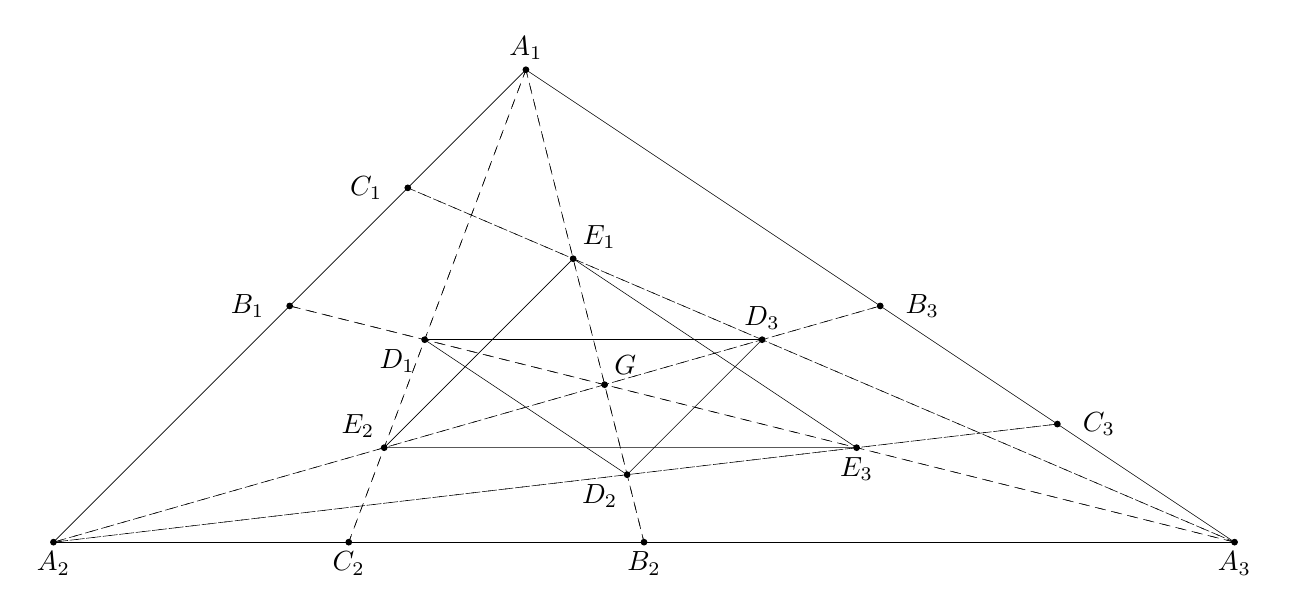
\begin{tikzpicture}[scale=3]
	% \useasboundingbox (-2,-2) rectangle  (2,2);
	\tkzDefPoint(0,2){A_1}
	\tkzDefPoint(-2,0){A_2}
	\tkzDefPoint(3,0){A_3}
	\tkzDefBarycentricPoint(A_1=1,A_2=1,A_3=1)\tkzGetPoint{G}
	\tkzDefBarycentricPoint(A_1=1,A_2=1)\tkzGetPoint{B_1}
	\tkzDefBarycentricPoint(A_2=1,A_3=1)\tkzGetPoint{B_2}
	\tkzDefBarycentricPoint(A_3=1,A_1=1)\tkzGetPoint{B_3}
	\tkzDefBarycentricPoint(A_1=1,B_1=1)\tkzGetPoint{C_1}
	\tkzDefBarycentricPoint(A_2=1,B_2=1)\tkzGetPoint{C_2}
	\tkzDefBarycentricPoint(A_3=1,B_3=1)\tkzGetPoint{C_3}
	\tkzInterLL(A_1,C_2)(B_1,A_3)\tkzGetPoint{D_1}
	\tkzInterLL(A_2,C_3)(B_2,A_1)\tkzGetPoint{D_2}
	\tkzInterLL(A_3,C_1)(B_3,A_2)\tkzGetPoint{D_3}
	\tkzInterLL(A_1,B_2)(C_1,A_3)\tkzGetPoint{E_1}
	\tkzInterLL(A_2,B_3)(C_2,A_1)\tkzGetPoint{E_2}
	\tkzInterLL(A_3,B_1)(C_3,A_2)\tkzGetPoint{E_3}
	\tkzDrawSegments(A_1,A_2 A_2,A_3 A_3,A_1)
	\tkzDrawSegments[dashed](A_1,C_2 A_2,C_3 A_3,C_1 A_1,B_2 A_2,B_3 A_3,B_1)
	\tkzDrawSegments[dashed](B_1,A_3 B_2,A_1 B_3,A_2 C_1,A_3 C_2,A_1 C_3,A_2)
	\tkzDrawSegments(D_1,D_2 D_2,D_3 D_3,D_1)
	\tkzDrawSegments(E_1,E_2 E_2,E_3 E_3,E_1)
	\tkzDrawPoints[fill=black](A_1,A_2,A_3,B_1,B_2,B_3,C_1,C_2,C_3,D_1,D_2,D_3,E_1,E_2,E_3,G)
	\tkzLabelPoints[above](A_1,D_3)
	\tkzLabelPoints[right=0.2](B_3,C_3)
	\tkzLabelPoints[below](A_2,A_3,B_2,C_2,E_3)
	\tkzLabelPoints[left=0.2](B_1,C_1)
	\tkzLabelPoints[above left](E_2)
	\tkzLabelPoints[above right](E_1,G)
	\tkzLabelPoints[below left](D_2,D_1)
	\end{tikzpicture}
\end{center}		
\end{figure}
We use Menelause's \thm\ on the following sets of points $\left\{\{A_1 E_2 C_2\},\{A_2 E_3 C_3\},\{A_3 E_1 C_1\}\right\}$ to get that
\begin{flalign}
&&\frac{GE_1}{E_1 A_1}&=\frac{GE_2}{E_2 A_2}=\frac{GE_3}{E_3 A_3}=\frac{2}{3}&\nonumber\\
&\Rightarrow&\frac{GE_1}{GA_1}&=\frac{GE_2}{GA_2}=\frac{GE_3}{GA_3}=\frac{2}{5}&\nonumber\\
&\Rightarrow&\frac{|\triangle E_1 E_2 E_3|}{|\triangle A_1 A_2 A_3|}&=\left( \frac{2}{5} \right)^{2}=\frac{4}{25} &\nonumber
\end{flalign}
We then use Menelause's \thm\ on the sets of points $\left\{\{A_1 D_2 B_2\},\{A_2 D_3 B_3\},\{A_3 D_1 B_1\}\right\}$ and then on the sets of points $\left\{\{A_1 G C_2\},\{A_2 G C_3\},\{A_3 G C_1\}\right\}$ to get that
\begin{flalign}
&&\frac{D_1 C_2}{A_1 D_1}&=\frac{D_2 C_3}{A_2 D_2}=\frac{D_3 C_1}{A_3 D_3}=\frac{3}{4}&\nonumber\\
&\Rightarrow&\frac{A_1 C_2}{A_1 D_1}&=\frac{A_2 C_3}{A_2 D_2}=\frac{A_3 C_1}{A_3 D_3}=\frac{7}{4}&\nonumber\\
&\Rightarrow&\frac{D_1 G}{G A_3}&=\frac{D_2 G}{G A_1}=\frac{D_3 G}{G A_2}=\frac{2}{7}&\nonumber\\
&\Rightarrow&\frac{|\triangle D_1 D_2 D_3|}{|\triangle A_1 A_2 A_3|}&=\left( \frac{2}{7} \right)^{2}=\frac{4}{49} &\nonumber\\
&\Rightarrow&\frac{|\triangle D_1 D_2 D_3|}{|\triangle E_1 E_2 E_3|}&=\frac{25}{49} &\nonumber
\end{flalign}

\qed

\clearpage

\item[4.]  Let $x = a^{2/3}, y = b^{2/3}$ and $z = c^{2/3}$. By a well-known special case of Schur's inequality, we have
\begin{equation*}
    x^3  + y^3 + z^2 + 3xyz \geq xy(x+y) + yz(y+z) + zx(z+x)
\end{equation*}
By AM-GM, we also have
\begin{equation*}
    xy(x+y) = x^2y + xy^2 \geq 2 \sqrt{x^2 y \cdot xy^2} = 2 x^{3/2} y^{3/2}
\end{equation*}
and similarly for $yz(y+z)$ and $zx(z+x)$. We therefore obtain
\begin{align*}
    a^2 + b^2 + c^2 + 3 &= x^3 + y^3 + z^3 + 3xyz \\
    &\geq xy(x+y) + yz(y+z) + zx(z+x) \\
    &\geq 2 x^{3/2} y^{3/2} + 2 y^{3/2} z^{3/2} + 2 z^{3/2} x^{3/2} \\
    &= 2(ab + bc + ca)
\end{align*}
which proves the inequality. \qed
\vspace{5mm}

\item[5.]  Assume for contradiction the problem claim does not hold, and let $p$ be the smallest (odd) prime not appearing in the sequence. We thus have that $p$ is not the least prime factor of 
$$1 + n \prod_{i=1}^n p_i^{i!}$$
for all $i$. Let $C$ be the smallest integer such that all primes less than $p$ appear in $p_1, p_2, \dots, p_C$. Thus, if $p$ divides $1 + n \prod_{i=1}^n p_i^{i!}$ for some $n > C$, then it must be the smallest factor.

Therefore, $p$ does not divide $1 + n \prod_{i=1}^n p_i^{i!}$ for all $i > C$. Now, define $T_m = \prod_{i=1}^m p_i^{i!}$. By Fermat's Little Theorem, we have for sufficiently high $i$ and $p_i$ (indeed, for $i > \textrm{max}(C, p-1)$), $p_i^{i!} \equiv 1$ (mod $p$). Thus, the residuce class of $T_m$ stays constant for sufficiently high $m$. Therefore, there exists an $m$ high enough such that $m T_m \equiv -1$ (mod $p$), noting that $T_m$ is not divisible by $p$. This proves that $p$ divides $1 + m T_m$, which is a contradiction. \qed


    

\end{enumerate}
\end{document}




